\newpage
\section{}

\subsection{Examine the Ni-Al-Ta ternary phase diagram, is there a strong temperature dependence?}

To evaluate eif there is a strong dependence on temperature, the Ni-Al-Ta ternary phase diagram was generated using the phase diagram tool at different temperatures, from $800^{\circ}$C to $1300^{\circ}$C, the resulting diagrams are shown in figure \ref{fig:diagram02}.

Figures \ref{fig:800C} and \ref{fig:900C} present the ternary phase diagram for the alloy at $800$°C and $900$°C respectively, from the diagrams it can be seen a small increase in the $\gamma$ phase  region. This can be noted in the $\gamma$ boundary line that moves from $xxx$ in figure \ref{fig:800C}, to $xxx$ Al fraction axis in figure \ref{fig:900C}.

\begin{figure}[h]
  \centering
  \subfloat[800°C\label{fig:800C}]{
    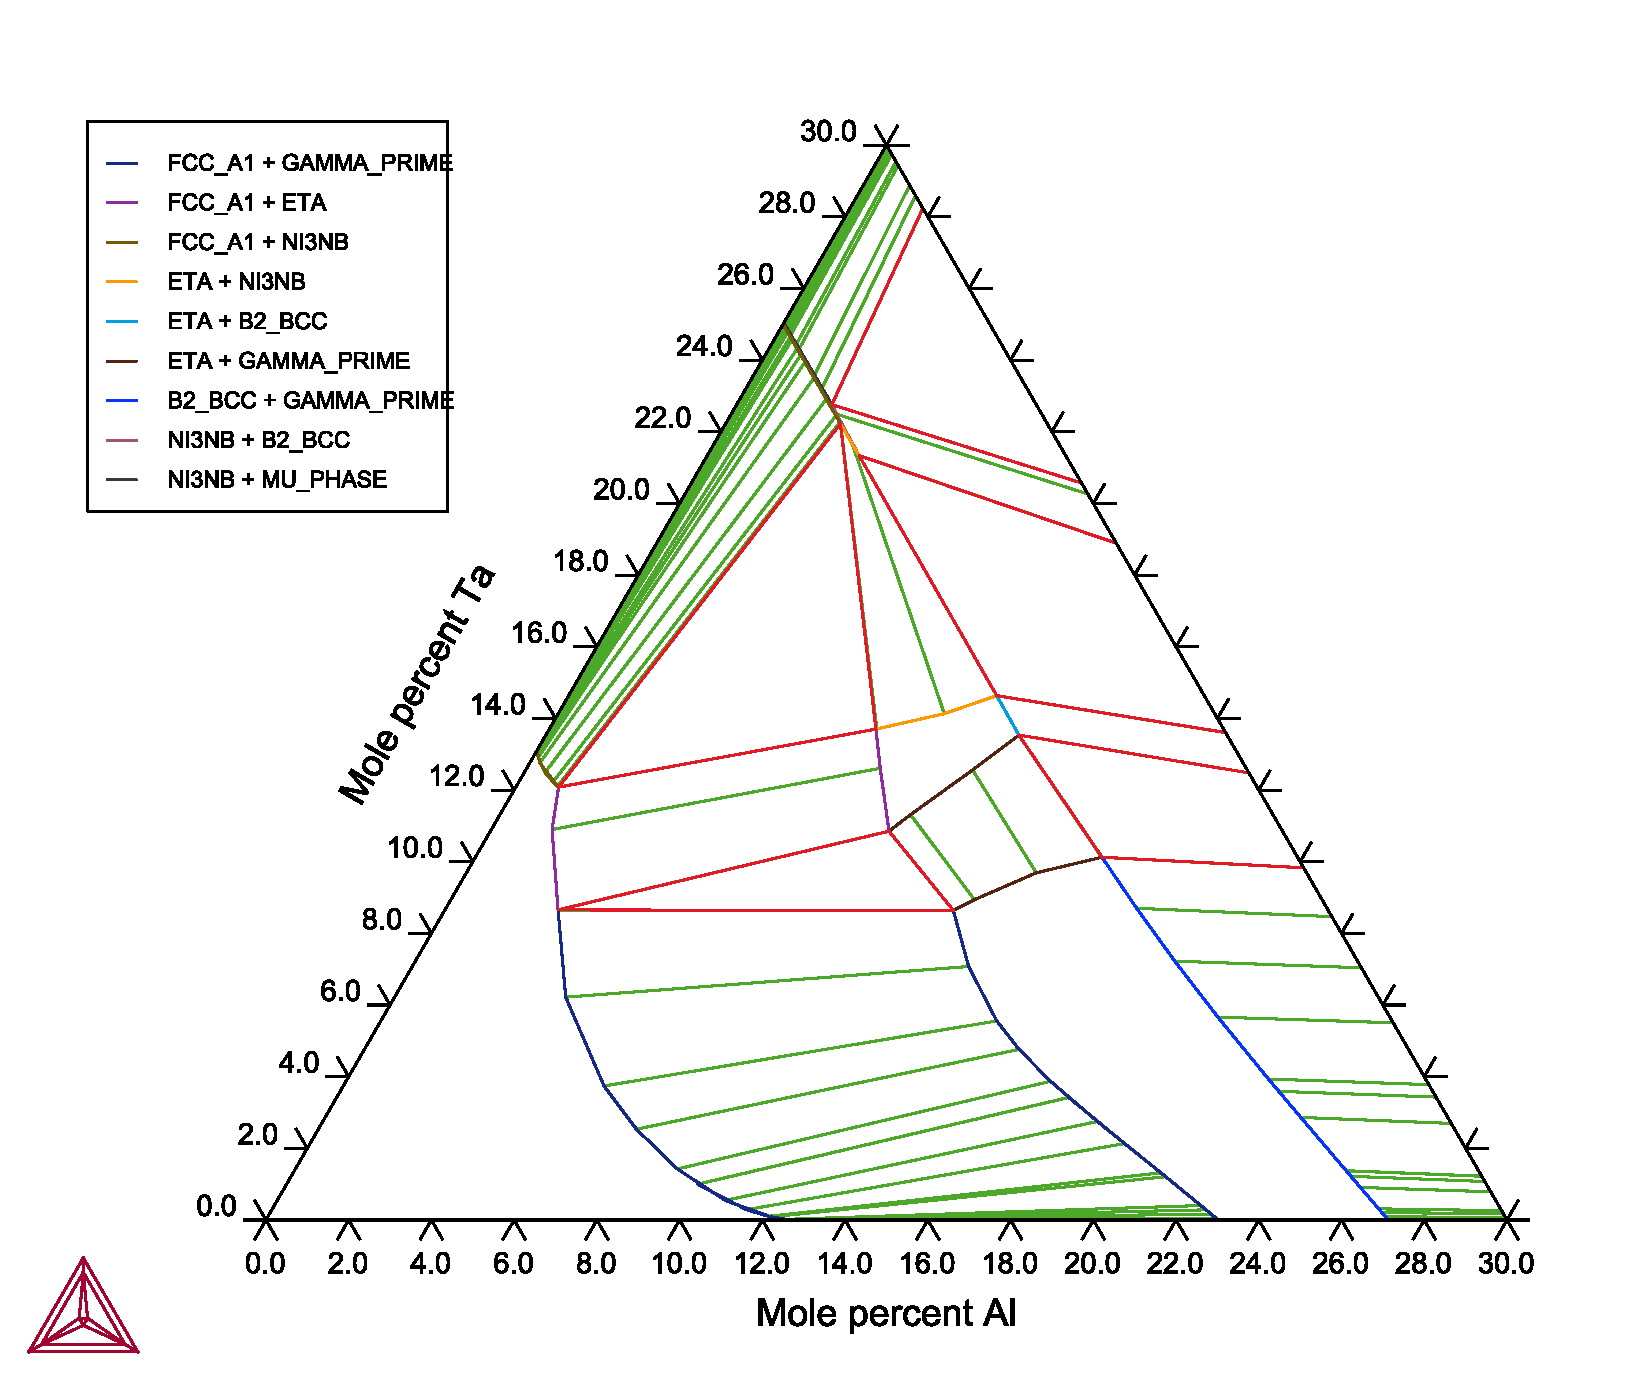
\includegraphics[width=0.5\textwidth]{graficas/Q2_NiAlTa_ternary_800C.pdf}
    }
  \subfloat[900°C\label{fig:900C}]{
    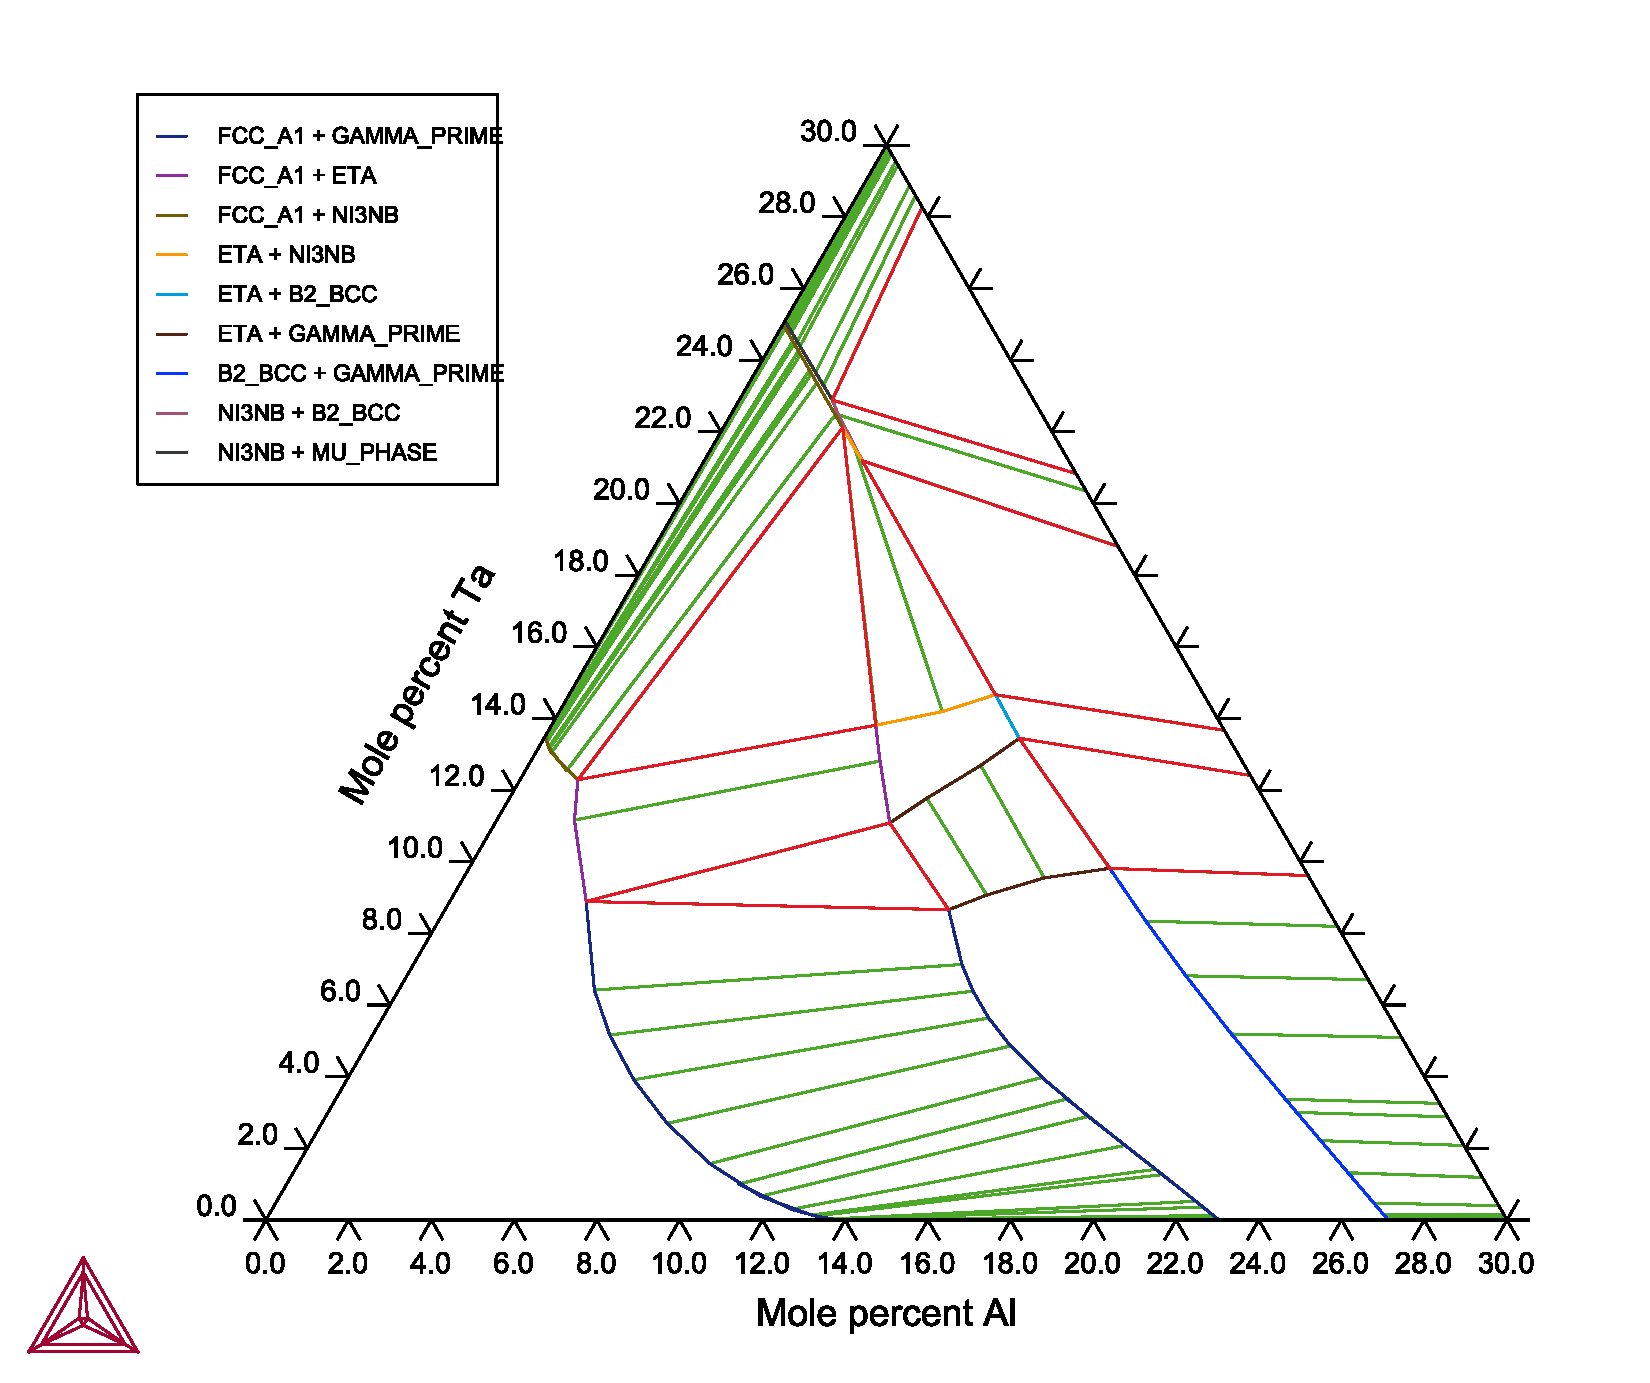
\includegraphics[width=0.5\textwidth]{graficas/Q2_NiAlTa_ternary_900C.pdf}
    }
  \caption{Ni-Al-Ta ternary diagram at different temperatures generated with \textit{ThermoCalc} \citep{thermocalc}}
  \label{fig:diagram02}
\end{figure}

As temperature increases, the increase on the $\gamma$ phase is more evident, where the bondary linw of the $\gamma$ phase moves from $xxx$ fraction at $10000$°C, in figure \ref{fig:1000C}, to $xxxx$ at $1100$°C, in figure \ref{fig:1100C}. There is also a decrease in the region of the $\gamma'$ phase; where the boundaries go from $yyy$ Al fraction to $yyy$. The change is more evident as the temperature increases to $1200$°C and $1300$°C, as it is shown in figures \ref{fig:1200C} and \ref{fig:1300C}; where the decrease of the region of $\gamma'$ phase is more evident. 

This indicates that there is a dependence on temperature on the equilibrium of the $gamma$ and $\gamma'$ phases in the Ni-Al-Ta alloy.

\begin{figure}[H]
  \centering
  \ContinuedFloat
  \subfloat[1000°C\label{fig:1000C}]{
    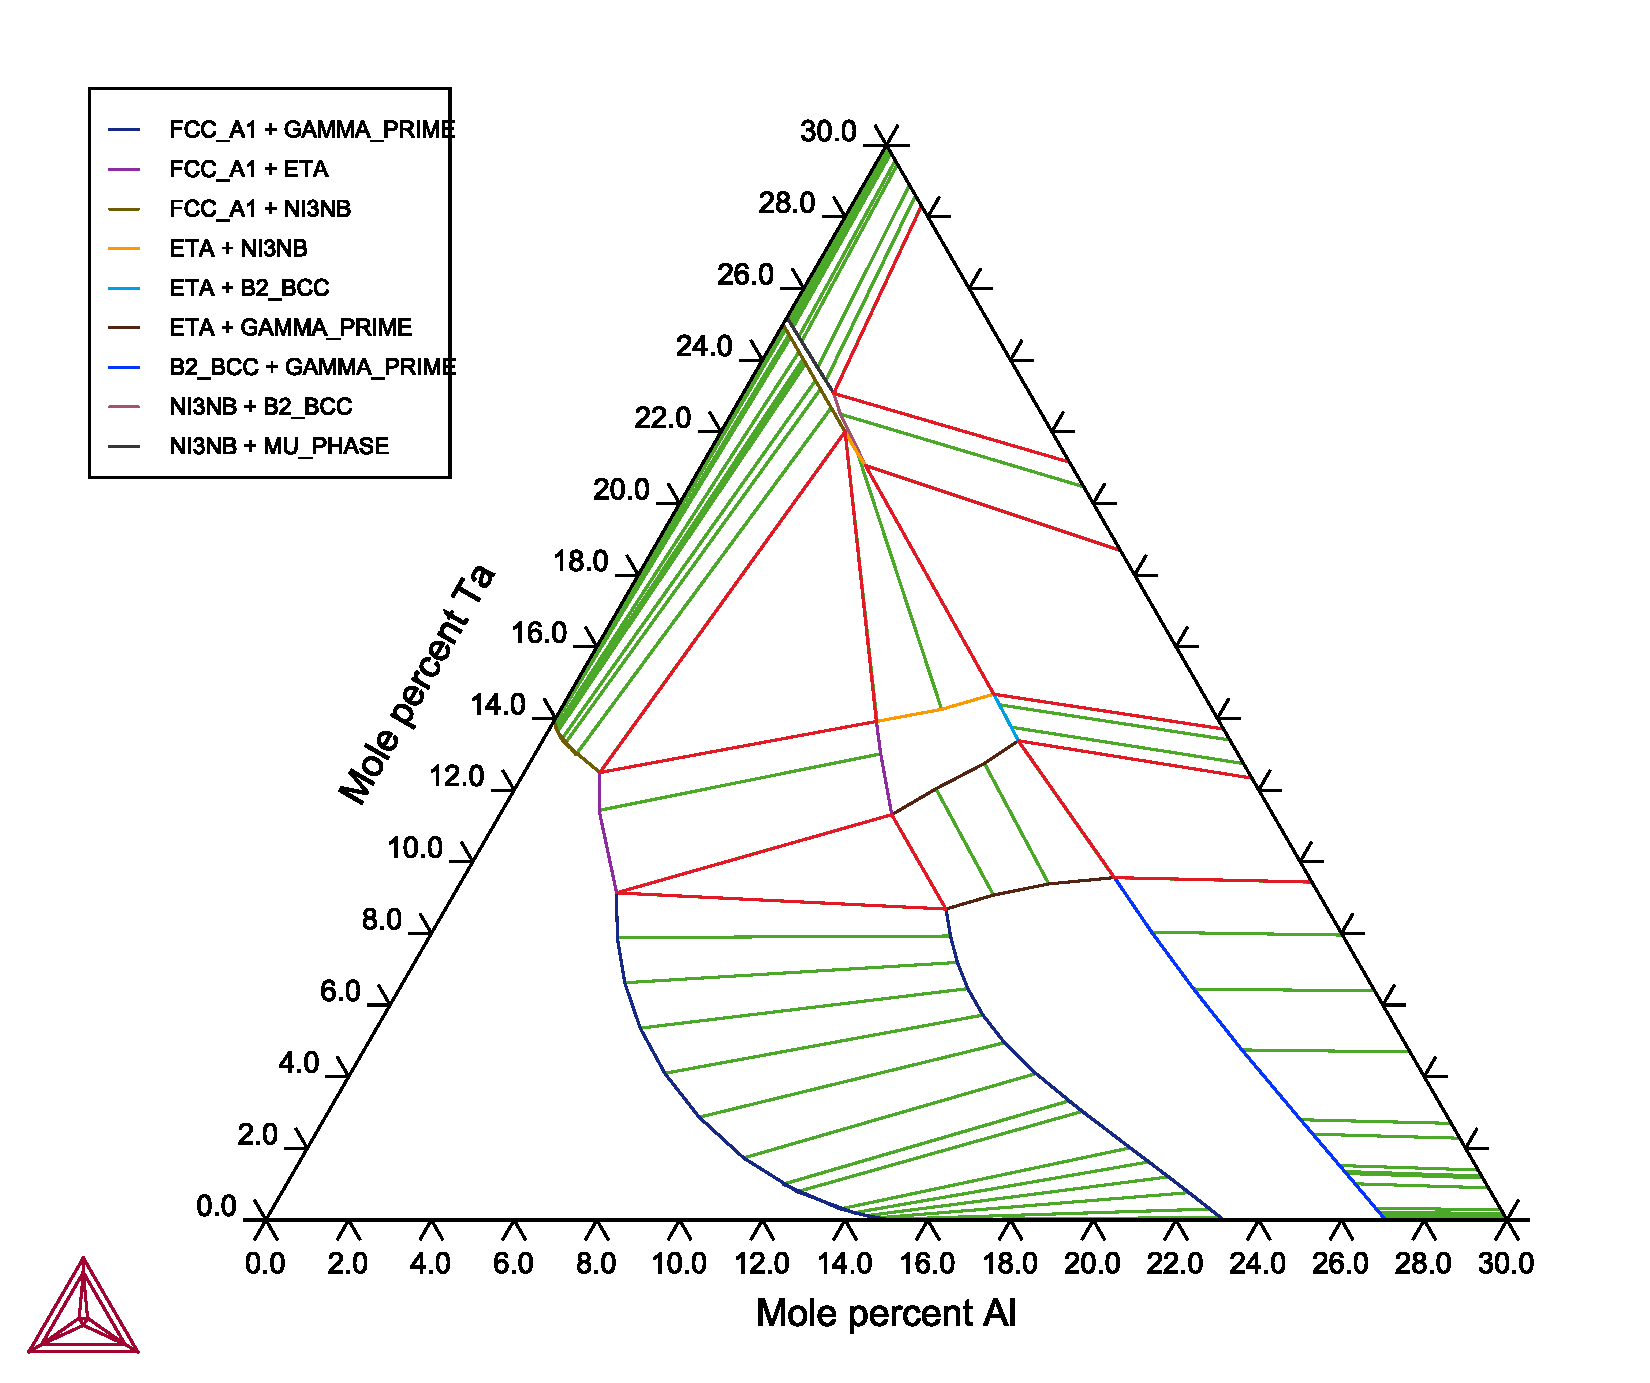
\includegraphics[width=0.5\textwidth]{graficas/Q2_NiAlTa_ternary_1000C.pdf}
    }
  \subfloat[1100°C\label{fig:1100C}]{
    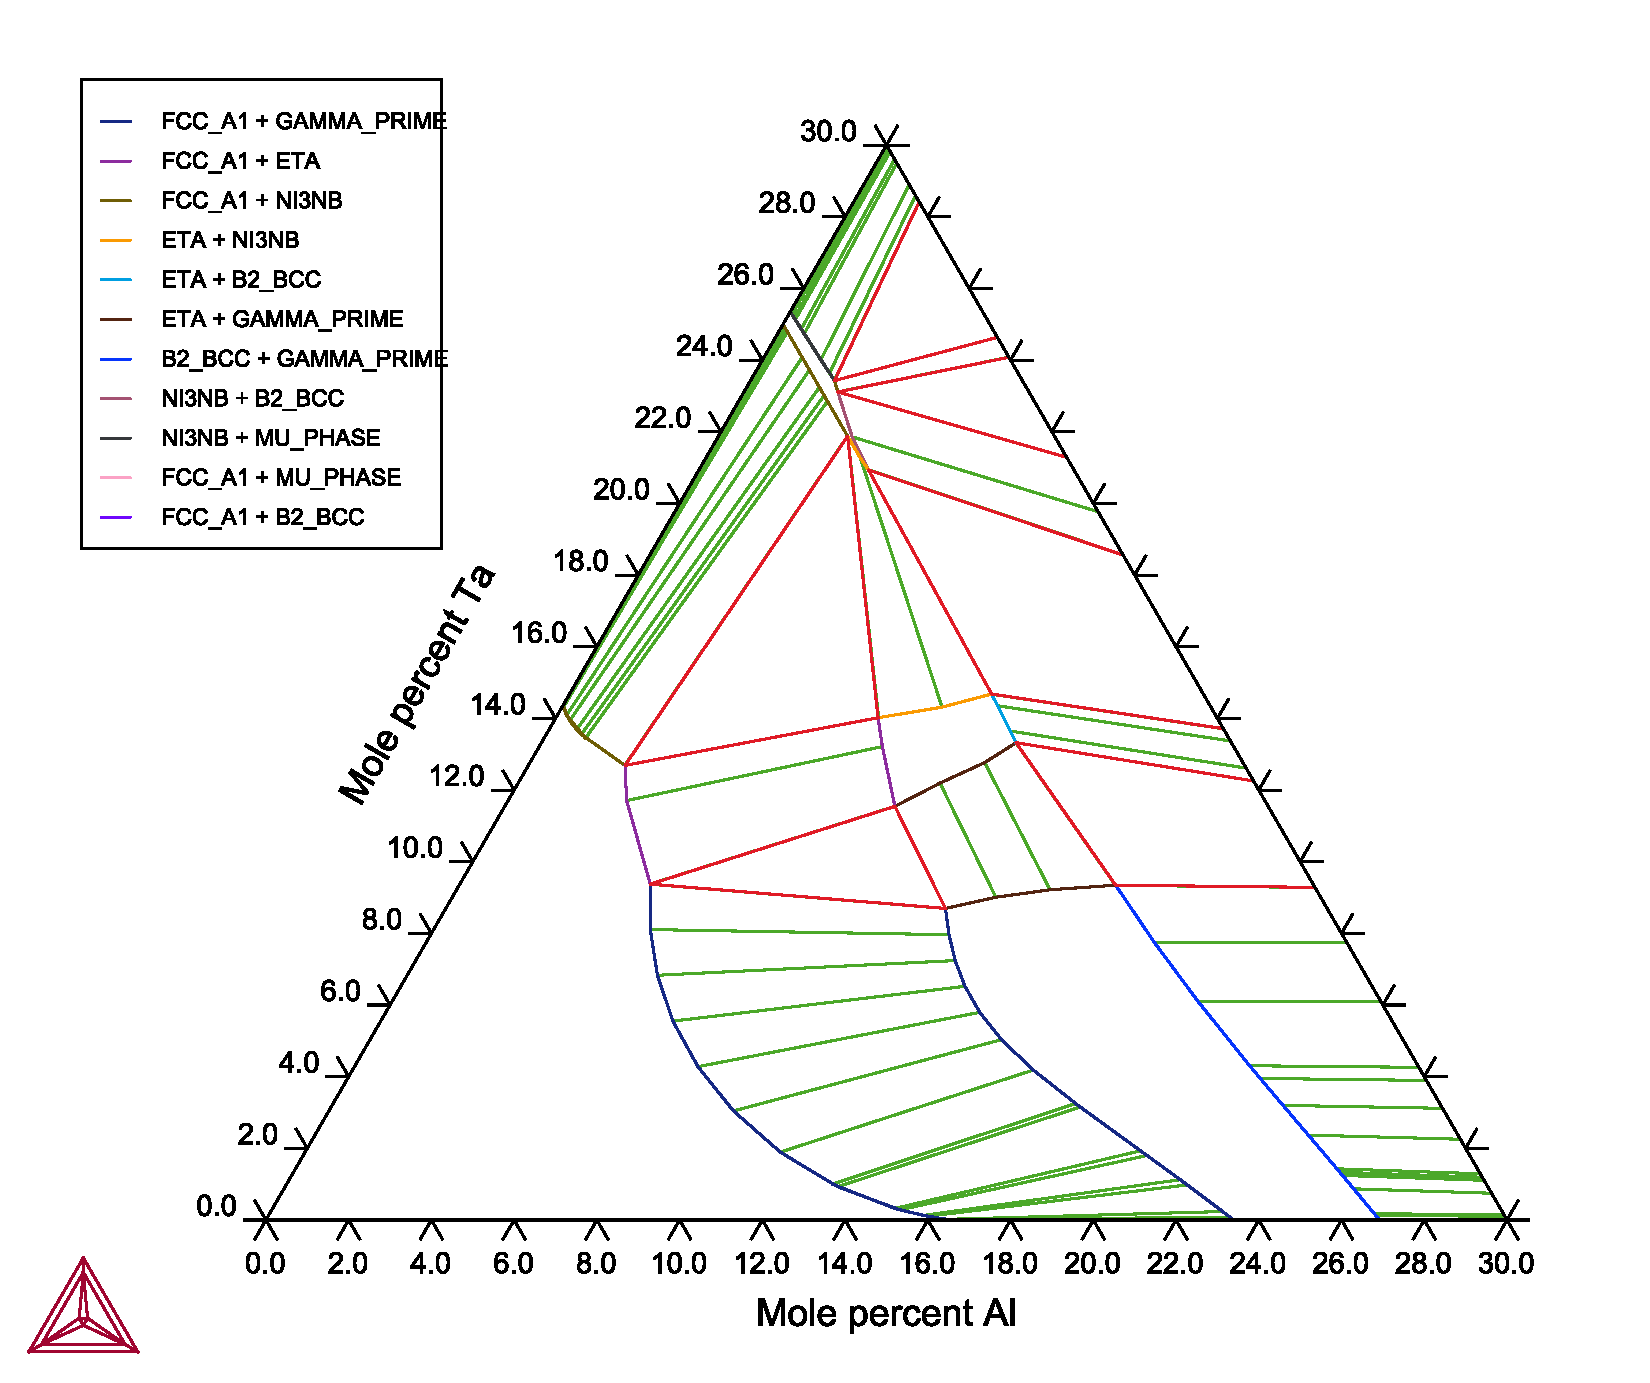
\includegraphics[width=0.5\textwidth]{graficas/Q2_NiAlTa_ternary_1100C.pdf}
    } \\
  \subfloat[1200°C\label{fig:1200C}]{
    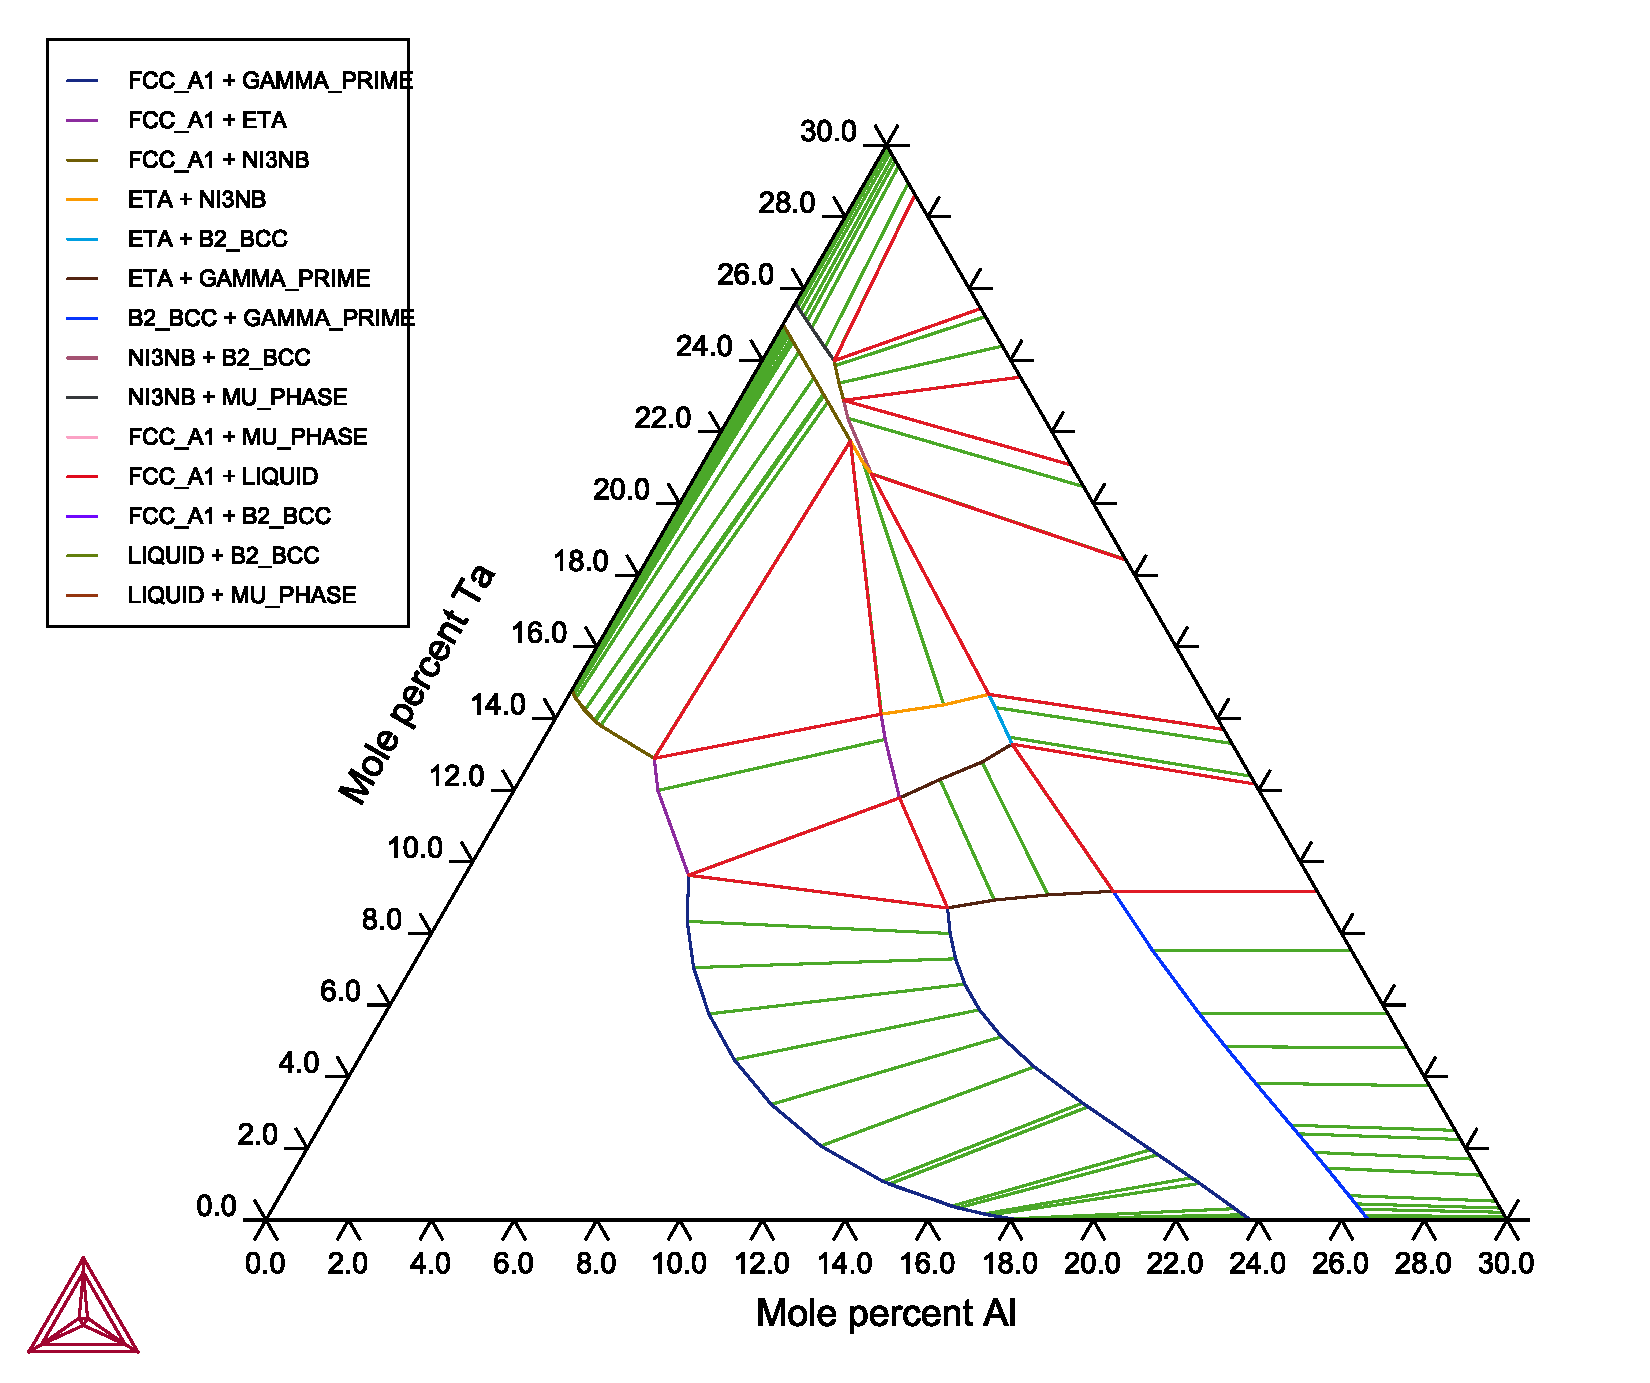
\includegraphics[width=0.5\textwidth]{graficas/Q2_NiAlTa_ternary_1200C.pdf}
    }
  \subfloat[1300°C\label{fig:1300C}]{
    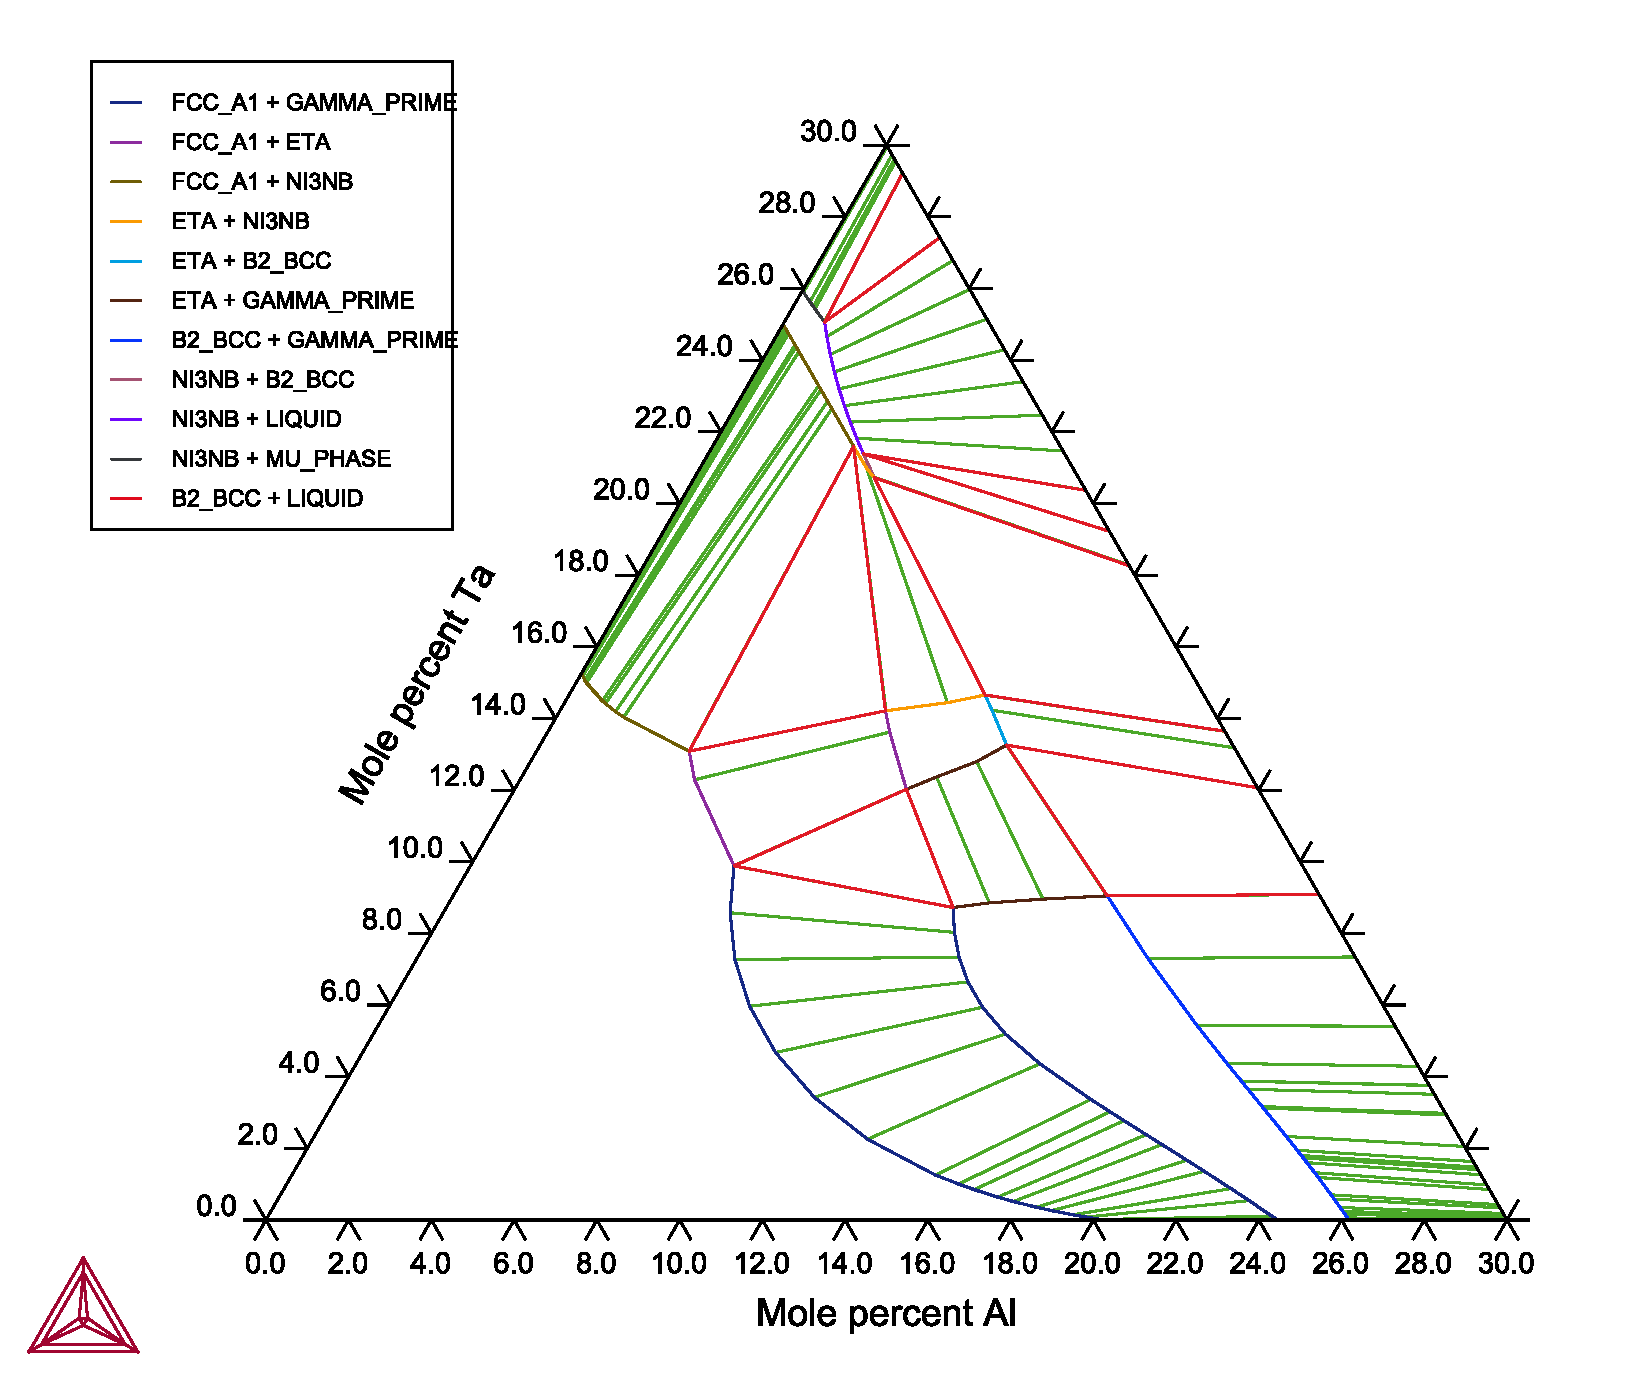
\includegraphics[width=0.5\textwidth]{graficas/Q2_NiAlTa_ternary_1300C.pdf}
    }
  \caption[]{\centering Ni-Al-Ta ternary diagram at different temperatures generated with \textit{ThermoCalc} \citep{thermocalc} (continued)}
\end{figure}



\newpage
\subsection{Ni-Al-Ta alloys for which $\gamma'$ phase fraction is optimal}

The optimal fraction is that for which $\gamma'$ is $75\%$. The 

\begin{table}[h]
  \centering
    \begin{tabular}{rrr}
        \multicolumn{1}{c}{\textbf{Mole percent Ni}} & \multicolumn{1}{c}{\textbf{Mole percent Al}} & \multicolumn{1}{c}{\textbf{Mole percent Ta}} \\ \hline \hline
        78.85099667 & 21.14900333 & 7.68378e-10 \\
        79.59362927 & 19.40637073 & 1 \\
        80.39594974 & 17.60405026 & 2 \\
        81.11631779 & 15.88368221 & 3 \\
        81.63158462 & 14.36841538 & 4 \\
        81.90005914 & 13.09994086 & 5 \\
        81.93775742 & 12.06224258 & 6 \\
        81.78294354 & 11.21705646 & 7 \\
        81.47817335 & 10.52182665 & 8 \\
        81.15616469 & 10.05173194 & 8.792103367
    \end{tabular}
  \caption{Results obtained from the }
  \label{tab:tab02}
\end{table}

\begin{figure}[h]
  \centering
  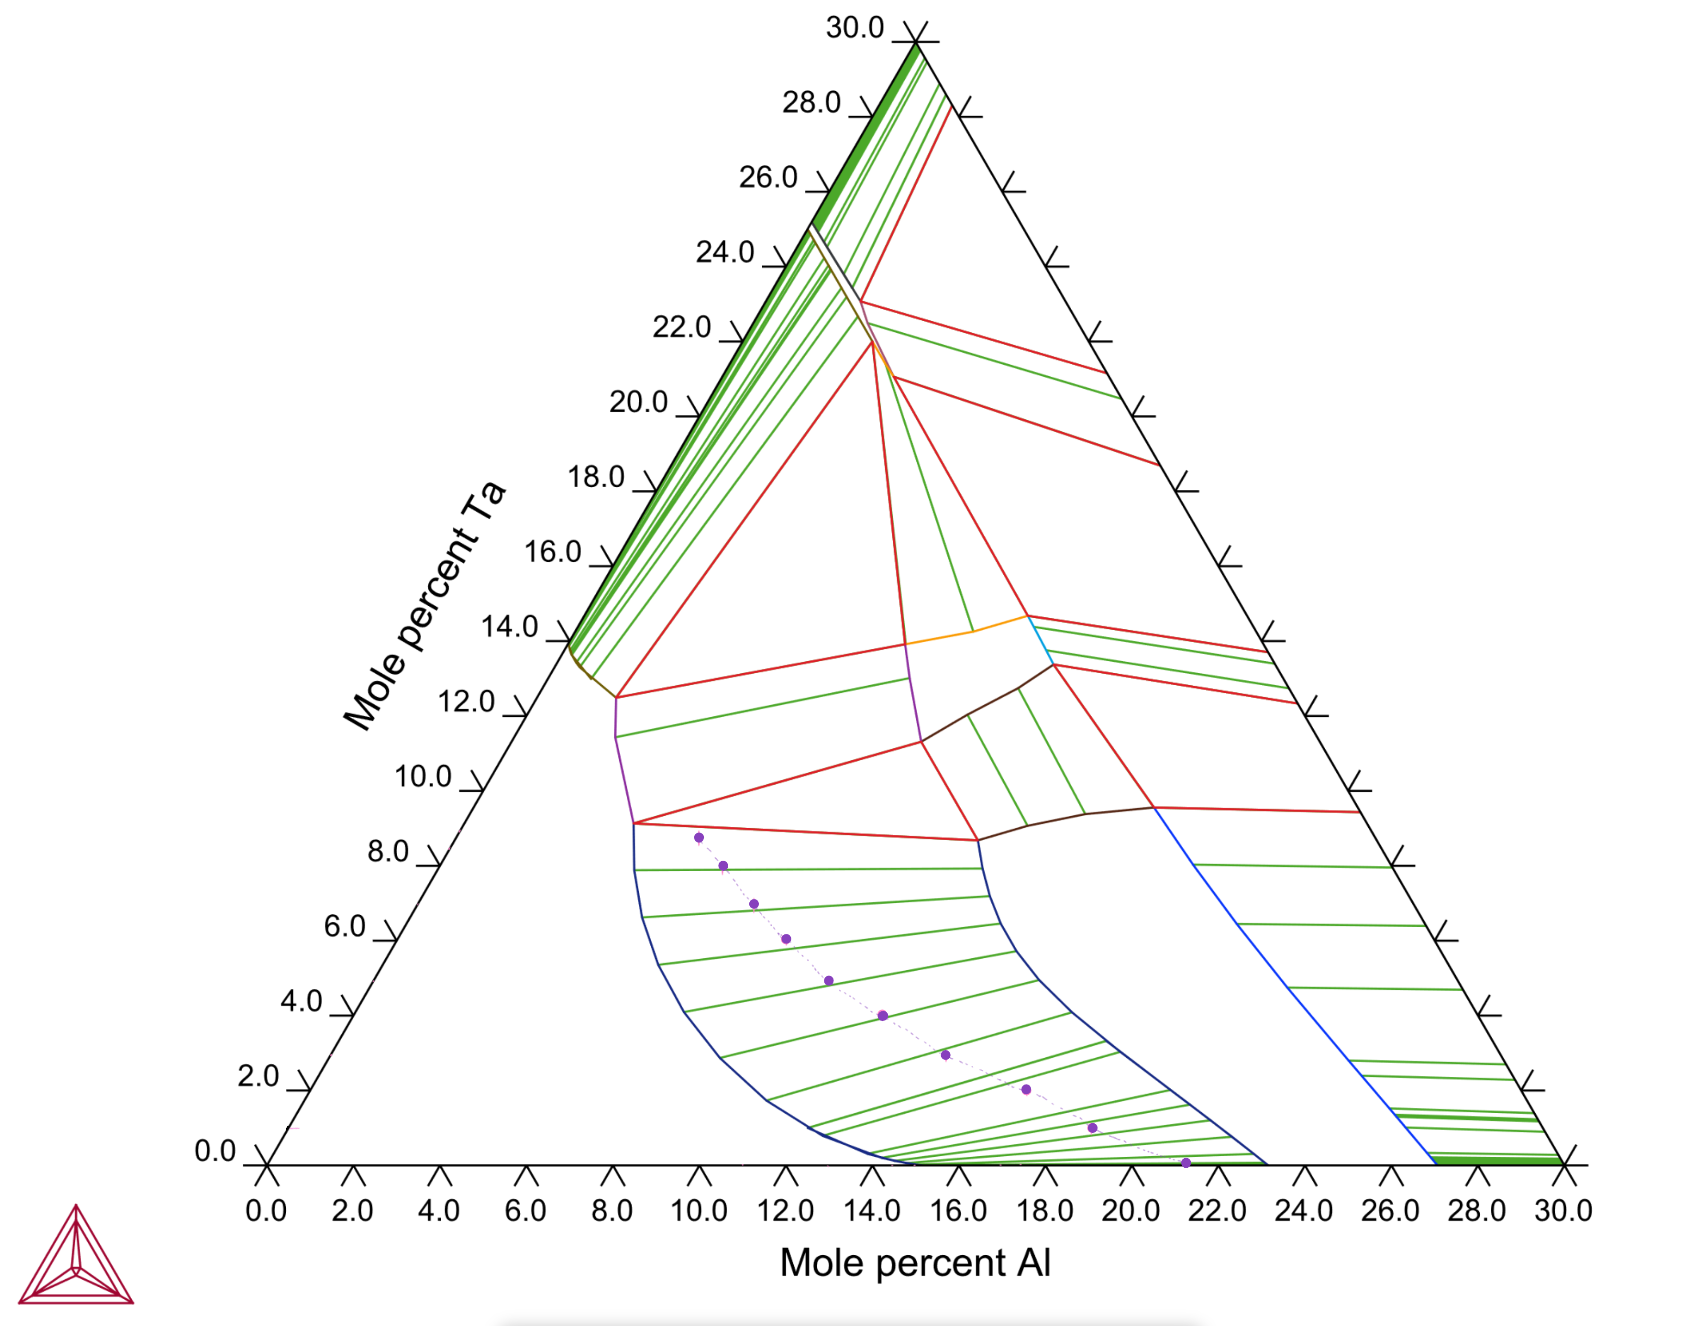
\includegraphics[width=0.95\textwidth]{graficas/Q2_NiAlTa_ternary03.png}
  \caption{Ni-Al-Ta ternary phase diagram with compositions for optimal $\gamma'$ phase fraction, $75\%$, generated using \textit{ThermoCalc} \citep{thermocalc}.}
  \label{fig:diagram03}
\end{figure}